
%\subsection{}

\begin{frame}{In an Ideal World}
When exploring the effect of something
  \begin{itemize}
  \item We would have a large dataset that...
  \begin{itemize}
   \item Was obtained from a Randomized Controlled Trial (RCT)
   \item Would help answer a clearly defined question
   \item Had all the covariates of scientific interest
   \item Contained no missing data
  \end{itemize}
\item But this almost never happens!
  \end{itemize}
  \note{ASK IS THIS A PROBLEM!!}
\end{frame}

\begin{comment}
 
 %took out ``in reality'' slide
\begin{frame}{In Reality}

  \begin{itemize}
   \item RCT's are expensive and often unethical
   \begin{itemize}
    \item We often get retrospective observational data
    %\item Pulled from a database or historical records
   \end{itemize}

   \item The questions we have may not be answerable from the data on hand
   \begin{itemize}
    \item The data obtained often doesn't support the original question in mind
   \end{itemize}

   \item The covariates collected are out of our control
   \begin{itemize}
    \item Since often no control of experiment, no control over what is collected
   \end{itemize}

   \item Lots of missing data
   \begin{itemize}
    \item Since no control over how the data is collected, we can't guarantee that everything is collected
  % \item This issue is seemingly omnipresent in all types of data collection
   \end{itemize}

  \end{itemize}
  \note{hey!}

\end{frame}

\end{comment}

\begin{frame}{Is This a Problem?}

\begin{center}
 {\Huge{YES!}}
\end{center}
  \begin{itemize}
   \item Without an RCT, we can't be sure if differences in outcome is due to the treatment or something else
   \item Omitting important factors may bias our results
   \item With missing data, we will be throwing away data and biasing our results
  \end{itemize}


\end{frame}

\begin{frame}{The Solution}
This thesis aims to fix these problems by...
  \begin{itemize}
   \item Filling in missing data via multiple imputation
   \item Creating meaningful analytical models via survival analysis
   \item Getting a causal interpretation from observational data via propensity scores\\~\\
  \end{itemize}
Goal: To be able to apply methods to cancer data

\end{frame}


\section{Introducing the Data}
\begin{frame}{Plan For This Presentation}
  \begin{figure}[h!]
  \centering
    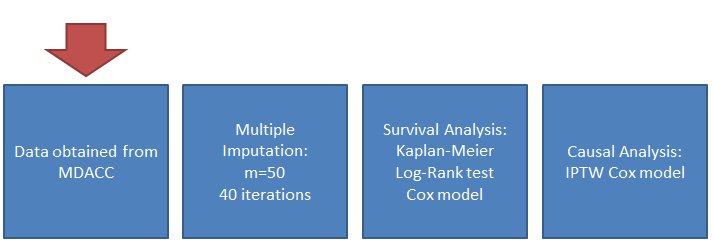
\includegraphics[width=0.9\textwidth]{data_flow}
\label{fig:data_flow}
\end{figure} 
\end{frame}

\subsection{Characteristics}

\begin{frame}{Data Explanation}
\begin{itemize}
 \item 1514 MD Anderson patients who had brain mets from breast cancer between October 2009 and 
 December 2012
 \item 1242 usable cases
 \item 90 covariates
 \begin{itemize}
  \item Missingness from 0 to 65\%
 \end{itemize}

\end{itemize}
\begin{table}[!ht]
\centering
\begin{tabular}{|c|c|}
\hline
Type                                                                            & Example                                                                       \\ \hline
Subject data                                                                    & Age range, race, date of birth                                                \\ \hline
Breast Cancer data                                                                     & TNM staging, type, receptor status                                            \\ \hline
\begin{tabular}[c]{@{}c@{}}Pre brain mets\\ data\end{tabular}                   & Treatment types                                                               \\ \hline
\begin{tabular}[c]{@{}c@{}}Post brain mets\\ clinical observations\end{tabular} & Seizures, headache, nausea                                                    \\ \hline
\begin{tabular}[c]{@{}c@{}}Post brain mets\\ data\end{tabular}                  & \begin{tabular}[c]{@{}c@{}}Treatment type, \\ type of brain mets\end{tabular} \\ \hline
Survival data                                                                   & Survival time after brain mets, censoring indicator                           \\ \hline
\end{tabular}
\caption{Data Categories and Examples}
\label{table:datacats}
\end{table}

\end{frame}

\subsection{Scientific Questions}
\begin{frame}{Questions of Interest}
Want to explore...
\begin{enumerate}
 \item Chemotherapeutic drugs: Capecitabine vs other chemotherapeutic agents
 \item HER2 directed therapies (Lapatinib, Trastuzumab) in HER2+ subjects \\~\\
 %  might want to move this later
 \end{enumerate}
 
 
 Note: treatment not determined at time of diagnosis 
 \begin{itemize}
  \item landmark (2 months) 
 \end{itemize}
 
\note{Human epidermal growth factor receptor 2 (HER2) overexpression drives the biology of 20
 pct of breast cancers, and predicts a poor prognosis for patients.}

\end{frame}


%%%%%%%%%%%%%%55
\subsection{Getting a feel for the data}
\begin{frame}{A Few Important Covariates}
  \begin{table}[!ht]
\centering
\adjustbox{max height=\dimexpr\textheight-5.5cm\relax,
           max width=\textwidth}{
\begin{tabular}{|c|c|c|}
\hline
Name        & \begin{tabular}[c]{@{}c@{}}Percent \\ Missing\end{tabular} & Meaning                                                                                                                                             \\ \hline
capeothno   & 18\%                                                        & \begin{tabular}[c]{@{}c@{}}Indicator: Capecitabine, other, or no chemotherapeutic\\ treatment. Treatment variable 1\end{tabular}                     \\ \hline
lapatrasno  & 18\%                                                        & \begin{tabular}[c]{@{}c@{}}Indicator: Lapatinib, Trastuzumab, or no HER2 treatment.\\ Treatment variable 2\end{tabular}                             \\ \hline
controlled  & 12\%                                                        & Indicator: Extracranial progression of brain mets                                                                                                   \\ \hline
%her2        & 10\%                                                        & Indicator: HER2 receptor status                                                                                                                     \\ \hline
hrher2      & 5\%   													& \begin{tabular}[c]{@{}c@{}}Categorical variable: The hormonal receptor and \\ HER2 receptor status of the subject\end{tabular}  						\\ \hline
braintype   & 4\%                                                        & Categorical: Single, multiple, Leptomeningeal disease                                                                                               \\ \hline                                                                       
timedx      & 1\%                                                        & \begin{tabular}[c]{@{}c@{}}Indicator: Time (years) from breast cancer diagnosis to brain\\ mets diagnosis greater or less than 6 years\end{tabular} \\ \hline
site5       & 1\%                                                     & Indicator: First metastasis was to brain                                                                                                            \\ \hline
race2       & 0\%                                                          & Categorical: White, Black, Hispanic, other                                                                                                          \\ \hline
priorn      & 0\%                                                          & \begin{tabular}[c]{@{}c@{}}Indicator: Number of prior treatments in metastatic setting \\ before brain mets\end{tabular}                            \\ \hline
os          & 0\%                                                          & Overall survival (months)                                                                                                                           \\ \hline
dead        & 0\%                                                          & Indicator: death indicator                                                                                                                          \\ \hline
agebrainmet & 0\%                                                        & Indicator: Age greater or less than 60 at time of brain mets                                                                                        \\ \hline

\end{tabular}
}
\caption{Table of important covariates to be used in the analysis}
\label{table:importantvars}

\end{table}
\end{frame}


\begin{frame}{Visualization of Missingness}
 \begin{figure}[h!]
  \centering
    \caption{Visualization of missingness in the cancer dataset}

    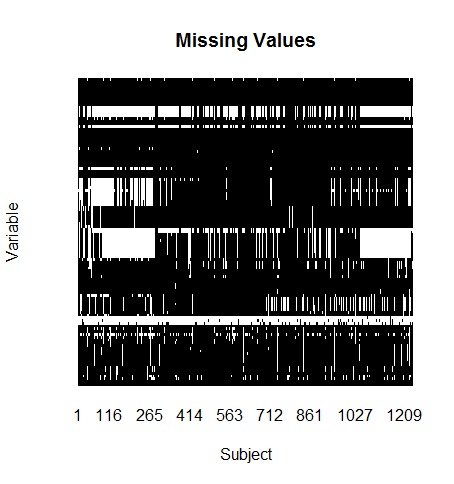
\includegraphics[width=0.55\textwidth]{missingvalues_plot.png}
\label{fig:missingplot}

\end{figure}
\end{frame}



%%%%%%%%%%%




\begin{comment}
 

\begin{frame}{Motivation}
\begin{itemize}
   \item This thesis is motivated by cancer survival data with moderate missingness
   \item We will build the theory for dealing with this situation
   \item And then apply it to a cancer data set
  \end{itemize}


\end{frame}

\begin{frame}{Abstract}
In this thesis, multiple imputation, survival analysis, and propensity score analysis are combined in 
order to answer questions about cancer data with moderate missingness. While each of these fields have 
been studied individually, there has been little work and analysis on using the three in trio.
Starting with an incomplete dataset, we aim to impute the missing data, run survival analysis on each
of the imputed datasets, and then do propensity score analysis to observe causal effects.
Along the way, many theoretical and analytical decisions are made. I explain why each decision is made, 
and offer ample evidence for the other choices such that the interested reader may implement the methods
if they so choose. I apply the methodology to a cancer survival dataset in a case study, but the methods 
used are general, and could be adapted for any type of data.
 
\end{frame}
\end{comment}
